% Example: a KAS bachelor's thesis in Czech, with Chinese and Japanese.
% Build with `make DOC=example-kas` (LuaLaTeX + biber, then the character
% count), or see README.md for the commands without make.
\documentclass[department=kas, type=ba, language=czech, gender=f, bib=apa]{upolthesis}
% KAS defaults: Times New Roman (or TeX Gyre Termes) 12 pt, 25 mm margins,
% 1.5 line spacing, no logo, cjk={zh,ja,ko}.  Plain Han characters are set
% as Chinese; use \textja{...} for Japanese kanji without kana.

\usepackage{booktabs}
\usepackage{pgfplots}
\pgfplotsset{compat=1.18,
  /pgf/number format/assume math mode=true,  % numbers in the text font
  /pgf/number format/use comma}               % Czech decimal comma
\sisetup{group-separator={\,}, output-decimal-marker={,}}

\thesisbibfile{example-kas.bib}

\title{Čaj v~Číně a~Japonsku}
\titleen{Tea in China and Japan}
\author{Jana Nováková}
\supervisor{Mgr. Jan Novák, Ph.D.}
\thesisyear{2027}
\submissiondate{30.~dubna 2027}

% the annotation (about ten lines): aims, method, results
\abstractcs{Práce srovnává čajovou kulturu Číny a~Japonska. Jejím cílem je
  ukázat, jak se z~čínského zvyku pít čaj vyvinul japonský čajový obřad.
  Vychází z~klasických pramenů, zejména z~Lu Yuova \emph{Čajového kánonu},
  a~z~japonských textů o~cestě čaje. ...}
\keywordscs{čaj, Čína, Japonsko, čajový obřad, \emph{čchaj-tao}, \emph{sadó}}

% the résumé in English, 100-200 words; printed by \makeresume
\abstracten{This thesis compares the tea cultures of China and Japan. It
  asks how the Chinese habit of drinking tea, described by Lu Yu in the
  eighth century in his Classic of Tea, became the Japanese tea ceremony.
  The first part summarises the history of tea in China from the Tang
  dynasty to the Ming dynasty, with attention to the changes in how tea was
  prepared: boiled cakes, whisked powder, and finally steeped leaves. The
  second part follows the arrival of tea in Japan with Buddhist monks and
  its development into chanoyu under Sen no Rikyū. The third part compares
  the vocabulary of tea in both languages. The thesis shows that the
  Japanese ceremony preserves the older Chinese method of whisked powdered
  tea, which disappeared in China itself, and that its aesthetic owes as
  much to Zen Buddhism as to Chinese models.}
\keywordsen{tea, China, Japan, tea ceremony, chadao, chadō}

\acknowledgements{Děkuji vedoucímu práce za trpělivost a~cenné rady.}

\abbreviations{%
  \begin{tabular}{@{}ll@{}}
    čín. & čínsky \\
    jap. & japonsky \\
  \end{tabular}}

\editorialnote{Čínské výrazy přepisuji českou transkripcí, při prvním
  výskytu doplněnou pinyinem a~znaky, např. \emph{čchaj} (\emph{chá} 茶).
  Japonské výrazy přepisuji Hepburnovým systémem s~délkami vyznačenými
  čárkou nad samohláskou, např. \emph{sadó} (\emph{sadō} 茶道).
  Znaky uvádím ve zjednodušené podobě pro čínštinu a~v~japonské podobě
  pro japonštinu.}

\begin{document}
\makefrontmatter[lof,lot]

\chapter{Úvod}
Čaj (čín. 茶 \emph{chá}, jap. お茶 \emph{ocha}) je nápoj, který se z~Číny
rozšířil do Japonska \citep{Okakura:1906}. Lu Yu (陆羽) jej popsal ve
\emph{Čajovém kánonu} (茶经 \emph{Chájīng}) \citep{LuYu:1974}.

\chapter{Čaj v~Číně}
\section{Čajový kánon}
Delší citát v~čínštině se láme do řádků sám:

\begin{quote}
茶者，南方之嘉木也。一尺、二尺乃至数十尺。其巴山峡川，有两人合抱者，伐而掇之。
\end{quote}

\section{Způsoby přípravy}
Tabulka~\ref{tab:priprava} shrnuje vývoj přípravy čaje.

\begin{table}[htbp]
  \centering
  \begin{tabular}{l l l}
    \toprule
    Dynastie & Způsob přípravy & Výraz \\
    \midrule
    Tang  & vařené lisované cihly & 煮茶 \emph{zhǔchá} \\
    Song  & šlehaný práškový čaj & 点茶 \emph{diǎnchá} \\
    Ming  & louhované lístky     & 泡茶 \emph{pàochá} \\
    \bottomrule
  \end{tabular}
  \caption{Způsoby přípravy čaje v~Číně}
  \label{tab:priprava}
\end{table}

\chapter{Čaj v~Japonsku}
Japonský čajový obřad (\textja{茶道} \emph{sadó}, také 茶の湯 \emph{čanoju})
uchovává čínský způsob šlehaného práškového čaje (Obrázek~\ref{fig:dovoz}).

\begin{figure}[htbp]
  \centering
  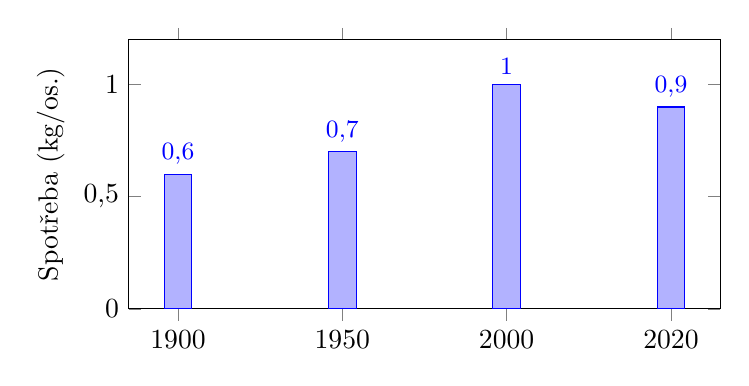
\begin{tikzpicture}
    \begin{axis}[ybar, width=.75\textwidth, height=5cm,
        symbolic x coords={1900,1950,2000,2020}, xtick=data,
        ylabel={Spotřeba (kg/os.)}, ymin=0, ymax=1.2,
        nodes near coords, every node near coord/.append style={font=\small}]
      \addplot coordinates {(1900,0.6) (1950,0.7) (2000,1.0) (2020,0.9)};
    \end{axis}
  \end{tikzpicture}
  \caption{Spotřeba čaje v~Japonsku (smyšlená data)}
  \label{fig:dovoz}
\end{figure}

\chapter{Závěr}
Text.

\makeresume

\thesisbibliography

\appendix
\chapter{Čajové náčiní}
\begin{tabular}{@{}lll@{}}
  \toprule
  Česky & Japonsky & \\
  \midrule
  čajová miska & \emph{čawan}  & \textja{茶碗} \\
  metlička     & \emph{časen}  & \textja{茶筅} \\
  \bottomrule
\end{tabular}

\end{document}
